\newcommand{\dirname}{\lstinline'sample-handout'}
\newcommand{\tgzname}{\dirname \lstinline'.tgz'}

\section*{Completing a Programming Assignment}

In this section, we'll walk through the steps of downloading,
completing, and submitting a programming assignment. You'll do this
for each assignment, so come back here if you get confused.

\begin{part}\TAGS{unix}
  Download the handout for this sample assignment by going to
  \autolab{} (\href{\autolabURL}{\autolabURL}), clicking on ``Sample
  Assignment (UNGRADED)'' and then on ``Download handout''.

\begin{colorpar}{clustercomputer}
\textbf{\em If you are on a GHC cluster computer}, this will save the
  handout as the file\linebreak[4] \tgzname{} in the 'Downloads'
  directory. We want to move it over to your 15-122 directory.
  The \lstinline'cp' command \textbf{\color{red} c}o\textbf{\color{red} p}ies files. You tell it
  where the file currently is (the ``source'') and then where you want the
  file to go (the ``destination''). Open a new terminal and run:
\begin{flalign*}
\lstinline'\% cp '&
\texttt{ }
\underbrace{\lstinline'Downloads/sample-handout.tgz'}_{\text{source}}
\texttt{ }
\underbrace{\lstinline'private/15122/'}_{\text{destination}}&
\end{flalign*}
Back to the terminal where you're in the \lstinline'private/15122' directory,
run \underline{\lstinline'ls'} to see the file:
\begin{lstlisting}[language={[coin]C}, belowskip=0pt]
% ls
sample-handout.tgz
\end{lstlisting}
\end{colorpar}

\enlargethispage{5ex}
\begin{colorpar}{laptop}
\textbf{\em If you are on your own laptop}, you will need to transfer
the file \tgzname{} to andrew so that you can work on it on that
system.

\smallskip

\begin{tabular}{|p{0.97\linewidth}|}
\hline
\textbf{\em If you are on a Mac or a Linux laptop}, open a new terminal
and \underline{\lstinline'cd'} to the directory where your browser
saved \tgzname{} (it's probably ``Downloads'').

We'll use the \underline{\lstinline'scp'} command to copy the file
from your laptop to the Andrew servers.  \underline{\lstinline'scp'}
is for \textbf{\color{red}s}ecurely
\textbf{\color{red}c}o\textbf{\color{red} p}ying files over a
network. You tell it where the file is now (the ``source'') and then
where you want the file to go (the ``destination''). Run the command
$$
\lstinline'% scp '
\texttt{ }
\underbrace{\lstinline'sample-handout.tgz'}_{\text{source}}
\texttt{ }
\underbrace{
    \underbrace{\lstinline'your\_id@unix.andrew.cmu.edu'
}_{\text{the computer we're sending the file to}}
\lstinline{:}
\underbrace{\lstinline'private/15122/'
}_{\text{where to put the file}}
}_{\text{destination}}
$$
It will ask for your andrew password.  Once you enter it, it will
transfer the file to andrew. Go back to the terminal where you're
\underline{\lstinline'ssh'}'d to andrew and in the \lstinline'private/15122'
directory. Run \underline{\lstinline'ls'} to see the file we just transferred:
\begin{lstlisting}
% ls
sample-handout.tgz
\end{lstlisting}
\vspace*{-3.5ex}~
\\\hline
\end{tabular}

\begin{tabular}{|p{0.97\linewidth}|}
\hline
\textbf{\em If you are on a Windows laptop},
you can use the pane on the left side to navigate the directories
on the machine you're \lstinline'ssh''d to.
 Double click on
``private'' and then ``15122'', and then you should see something like
this:

\begin{wrapfigure}[5]{L}{0.22\textwidth}
\vspace{-2ex}
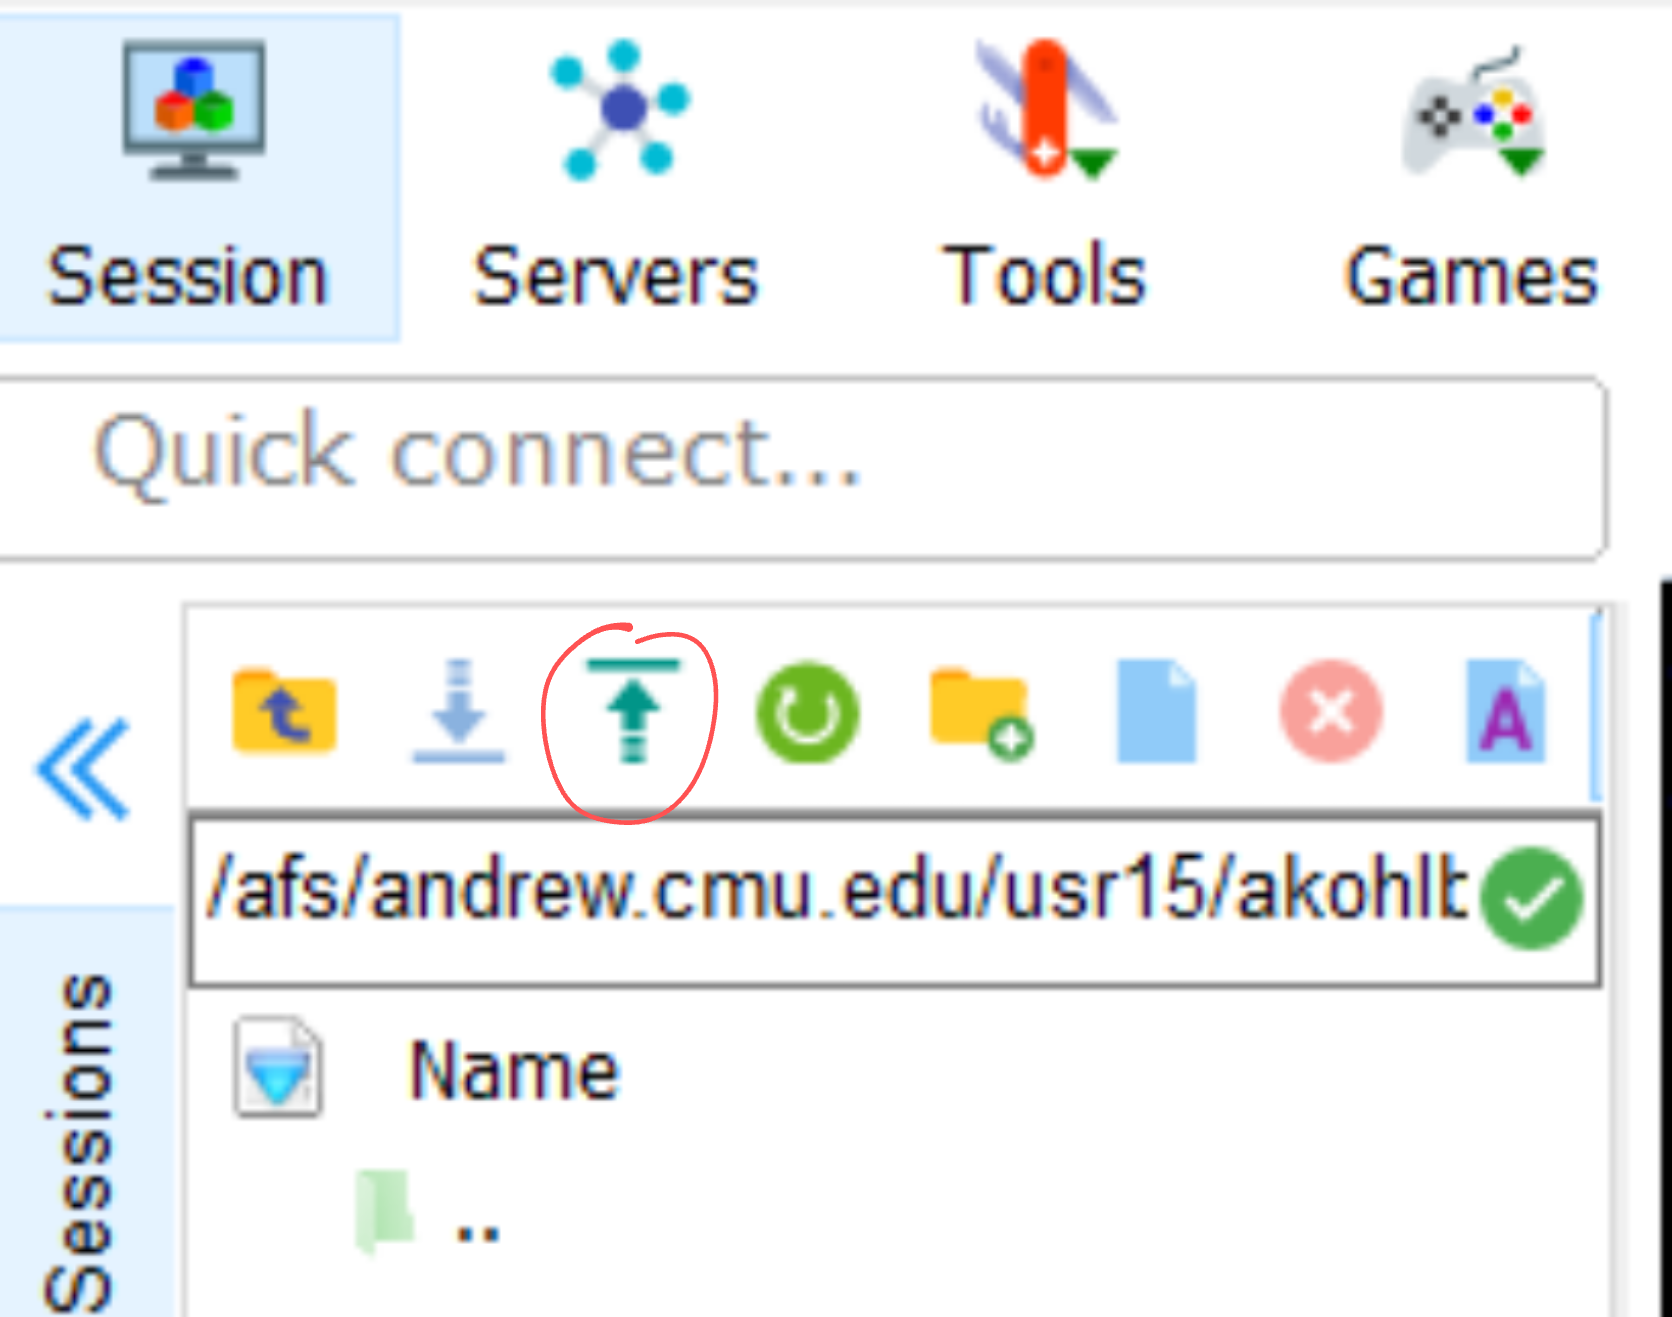
\includegraphics[width=\linewidth]{\img/moba3.png}
\end{wrapfigure}

Click on the circled button and select the \tgzname{} file from your
 computer to copy to the andrew machine.

Go back to the terminal where you're
\lstinline'ssh''d to andrew and in the \lstinline'private/15122'
directory. Run \lstinline'ls' to see the new file:
\begin{lstlisting}
% ls
sample-handout.tgz
\end{lstlisting}

Note that when navigating, clicking the two dots will move you up a
directory (for example, from \lstinline'15122' to \lstinline'private').
\\\hline
\end{tabular}
\end{colorpar}
\end{part}

\begin{part}\TAGS{unix}
\tgzname{} is a compressed archive (like a \lstinline'.zip' file)
consisting of
several files.  You can retrieve them with the following
command~\footnote{If this command fails, try %
\lstinline[basicstyle=\smallerbasicstyle]'tar xvf sample-handout.tgz'.}:
\begin{lstlisting}[language={[coin]C}]
% tar xfzv sample-handout.tgz
sample-handout/
sample-handout/factorial.c0
sample-handout/favorite_number.c0
sample-handout/README.txt
\end{lstlisting}

You've now created the directory \dirname{} containing the three files
\lstinline'README.txt', \lstinline'factorial.c0', and
\lstinline'favorite_number.c0'.  Go to this directory:

  \lstinline[language={[coin]C}]'% cd sample-handout'
\end{part}

\begin{part}\TAGS{unix}
  Verify you are in the \lstinline[language={[coin]C}]'sample-handout'
  directory by entering the command
  \underline{\lstinline[language={[coin]C}]'pwd'} to get the
    \textbf{\color{red}p}resent
  \textbf{\color{red}w}orking \textbf{\color{red}d}irectory and by entering the command
  \underline{\lstinline[language={[coin]C}]'ls'} to see the files in that
  directory.  You should see something like this with your andrew id
  instead of \lstinline[language={[coin]C}]'<your_id>':

\begin{lstlisting}[language={[coin]C}]
% pwd
/afs/andrew.cmu.edu/<usr_number>/<your_id>/private/15122/sample-handout
% ls
factorial.c0  favorite_number.c0  README.txt
\end{lstlisting}
\end{part}

\subsection*{Editing your program}

You can use any editor you wish to write and edit your programs, but
we highly recommend you try out \lstinline[language={[coin]C}]'vim'
and \lstinline[language={[coin]C}]'emacs' since these editors can do
much more than just help you edit your code (as you will see). For
this lab, \textbf{try both of them} by following the
instructions below.  Later, use the one you like best\footnote{
See the \href{http://www.cs.cmu.edu/~15122/about.shtml}{course website}
for some links to learn more about using these editors. They both
are capable of a lot more than we describe here.}.

\begin{part}\TAGS{unix}
  Open the file \lstinline[language={[coin]C}]'factorial.c0' that you
  downloaded from the previous part of the lab:

  \textbf{VIM:}\\ \lstinline[language={[coin]C}]'% vim factorial.c0'

  \textbf{EMACS:}\\ \lstinline[language={[coin]C}]'% emacs factorial.c0'
\end{part}

If a file doesn't exist, the editor will start with a new empty file.
You should see the editor start in the Terminal window, and you should
see a program that looks like it computes factorial. The program is
written in C0, the language we'll be using to start the semester.

\begin{part}\TAGS{unix}
  Edit the program and add your name and section letter at the
  appropriate locations. Use the instructions below for the editor
  you're using.

  \textbf{VIM:} This editor has two modes, \emph{insert mode} where
  you can insert text, and \emph{command mode} where you can enter
  commands.  It starts in command mode so you can't edit
  immediately. Use the arrow keys to move around the file. While in
  command mode, if you press ``\lstinline'i''', the editor changes you
  to insert mode, allowing you to type text. Go to insert mode and
  add your name and section letter.
  Press the Escape (ESC) key while in insert mode to return
  to command mode.

  \textbf{EMACS:} You can just start typing and editing without
  hitting special keys. You can use the arrow keys to navigate around
  the file to insert code. There are many shortcuts and built-in
  features to emacs but you don't need them right now. In the file,
  insert your name and your section letter in the appropriate comments
  in your program.

\end{part}

\begin{part}\TAGS{unix}
  Save your changes and exit the editor.

  \textbf{VIM:} Make sure you're in command mode by pressing ESC\@.
  Then, you can save your work and exit vim by entering the
  sequence ``\lstinline':wq''' followed by pressing Enter.
  (If you have unsaved changes you would like to discard,
  you'll have to enter the sequence ``\lstinline':q!''' followed by Enter.
  You can also save without exiting by entering the sequence
  ``\lstinline':w''' followed by Enter.)

  \textbf{EMACS:} Once you're ready to save, press Ctrl-x (the Control
  key and the ``\lstinline'x''' key at the same time) followed by
  Ctrl-s. You can exit by pressing Ctrl-x followed by Ctrl-c.  If you
  have not saved before exiting, Emacs will ask you whether you want
  to save your file (since you changed it) --- press ``\lstinline'y'''
  for yes. (Press ``\lstinline'n''' instead if you don't want to save
  your changes).

\end{part}

\begin{part}\TAGS{unix}
Try out your new editing skills on the file \lstinline'favorite_number.c0'.
You should see where the file tells you to add a line that returns your
favorite number, like this:
\begin{lstlisting}[language={[coin]C}, belowskip=0pt]
int my_favorite_number() {
    /* add a line below that returns your favorite number */
    return 17; // this is *my* favorite number. Choose your own.
}
\end{lstlisting}
\end{part}

\checkpoint*{\TAGS{compilation}}

Recall lab 1.  What command would you compile with to enable contract
checking in a file named \lstinline'fastpow.c0'?

\bigskip

\lstinline'prompt> '\answerline{cc0 -d fastpow.c0}

\begin{solutionFmt}
\clearpage
\end{solutionFmt}



\subsection*{Submitting Programming Assignments}
\begin{part}\TAGS{course-policies}
You will submit your \emph{programming} assignments
using \autolab{}, the site where you downloaded the handout
from.  Let's see how that works on the files \lstinline'factorial.c0'
and \lstinline'favorite_number.c0'.

We will always submit compressed files.  You do so by typing
the following at the Unix prompt:
\begin{lstlisting}[language={[coin]C}]
% tar cfzv handin.tgz factorial.c0 favorite_number.c0
\end{lstlisting}
The above command puts your files \lstinline'factorial.c0' and
\lstinline'favorite_number.c0' into a
compressed archive file named \lstinline'handin.tgz'.

\begin{colorpar}{clustercomputer}
\textbf{\em If you are on a GHC cluster machine}, you don't need to
do anything special.
\end{colorpar}

\begin{colorpar}{laptop}
\textbf{\em If you are on your own laptop}, you need to move the
\lstinline'handin.tgz' file from the andrew server back to your own
laptop.

\smallskip

\begin{tabular}{|p{0.97\linewidth}|}
\hline
\textbf{\em If your laptop is running Linux or Mac}, open a new terminal.
We'll use the \lstinline'scp' command from earlier.
$$
\lstinline[basicstyle=\smallbasicstyle]'% scp '
{}%\texttt{ }
\underbrace{
    \underbrace{\lstinline[basicstyle=\smallbasicstyle]'your\_id@unix.andrew.cmu.edu'
    }_{\text{the computer the file is on now}}
    \lstinline{:}
    \underbrace{\lstinline[basicstyle=\smallbasicstyle]'private/15122/sample-handout/handin.tgz'
    }_{\text{where the file is now}}
}_{\text{source}}
~%\texttt{ }
    \underbrace{\lstinline[basicstyle=\smallbasicstyle]'.'}_{\text{dest}}
$$
The \lstinline'.' at the end means ``here'' --- it tells \lstinline'scp'
to put the file in the current directory your terminal is in. If you
didn't \lstinline'cd' anywhere else, it's the home directory on your
laptop.
\\\hline
\end{tabular}

\begin{tabular}{|p{0.97\linewidth}|}
\hline
\textbf{\em If you are on a Windows laptop},
use the left-side pane again to navigate inside the \dirname{}
directory and click on the \lstinline'handin.tgz' file. Next
to the ``up'' button you used before is a corresponding
``down'' button. Click that, and select where to save the file
on your computer.
\\\hline
\end{tabular}
\end{colorpar}

Next, point your browser to \autolab, go to the sample assignment's
entry and upload the newly created file \lstinline'handin.tgz' using
the ``Submit File'' button.

\enlargethispage{5ex}
Check that you submitted the right file by clicking on the ``view
source'' icon.  \textbf{Always check your submissions!}

There's also an easier way to submit from an andrew computer.  You can
use the \lstinline'handin' command to \textbf{\color{red}hand in} your
work. The file \lstinline'README.txt' in each handout will tell you
how to submit using \lstinline'handin'. Look at the \lstinline'README'
for this sample homework to see what to do (you can view the file by
opening it in an editor, like Vim or Emacs).
%TODO write a readme for sample, add it to all the places we list the dir contents
\end{part}
